% !TeX spellcheck = en_US
\RequirePackage[l2tabu, orthodox]{nag}

\documentclass[paper=a4,
fontsize=13pt,
%cleardoubleplain,
%headsepline,
%liststotoc,
bibliography=totoc,
%parskip=half,
%pointlessnumbers,
twoside,
%openright, % only for print version
hidelinks,
openany, % no empty pages between chapters
%draft,
%smallheadings
]{scrbook}

\usepackage{marginfit}
\usepackage{setspace}

%For UBP
\usepackage{geometry}
\geometry{tmargin=27mm,bmargin=20mm,left=25mm,right=25mm, marginparwidth=14mm, marginparsep=2mm,bindingoffset=5mm}
\setlength{\footskip}{30pt}

\usepackage{etoolbox}

\setstretch{1.05} % line separation +1/+2 points

\clubpenalty10000
\widowpenalty10000
\displaywidowpenalty=10000

\makeatletter
\expandafter\patchcmd\csname\string\maketitle\endcsname{\if@twoside}{\iftrue}{}{}
\makeatother

%for consecutive footnote numbering in the complete document
\usepackage{chngcntr}
\counterwithout{footnote}{chapter}
\hfuzz=2pt

\setcounter{secnumdepth}{3}    % Number subsubsections in the chapters
\setcounter{tocdepth}{3}       % Put subsubsections in the table of contents
\usepackage{warning} % for warning messages

%Alternative to \input glyphtounicode.tex
%Enables copy and paste of ligatures, such as appearing in "workflow"
\usepackage{cmap}

\usepackage[ngerman,british]{babel} % language selection
\usepackage[T1]{fontenc} % western languages encoding
\usepackage[utf8]{inputenc} % set encoding to UTF-8
\DeclareUnicodeCharacter{1F3C6}{\faTrophy}

% \usepackage{cite}
\usepackage[sort&compress,square,numbers]{natbib}

\usepackage{longtable}

\usepackage{multicol}
\usepackage{multirow}

\usepackage[font=small]{caption}

\usepackage{environ}

% figures only appear after their first use, never ever before
\usepackage{flafter}

\usepackage{microtype} % nicer output
\usepackage{hfoldsty} % nicer output
\usepackage{lmodern} % use the modern fonts
\usepackage{charter} % use the charter font

\usepackage[final]{listings} % listings package fuer source code

\usepackage{epigraph} % citations at section start
\usepackage{rotating} % rotated images and tables
\usepackage{enumerate} % better enumeration environment
\usepackage{booktabs} % nice looking tables
\usepackage{amsmath,amssymb,amsfonts} % math extensions
\usepackage{marginnote} % notes on the margin of the page
\usepackage[sharp]{easylist} % lists denoted with the # symbol

\usepackage{mdframed} % show frames (borders)

\usepackage{ifthen} % if and then

\usepackage{dirtree} % folder structures

\usepackage{tocloft}

\usepackage{fontawesome}

\usepackage[automark]{scrpage2} % Kopf- und Fusszeilen-Format mit KOMA-Script

\usepackage{strict} % check for not using undefined environments

\usepackage[strict=true,english=american]{csquotes}

\usepackage[printonlyused]{acronym} % for spelled out acronyms
\usepackage{todonotes} % show todos in code

\usepackage{relsize} % Set the font size relative to the current font size
\usepackage{xspace} % Define commands that appear not to eat spaces

\usepackage{mfirstuc} % for capitalization

\usepackage{paralist} % compactenum, compactdesc and compactitem environments

\usepackage{multirow}
\usepackage{enumitem} % Control layout of itemize, enumerate, description
\usepackage{makeidx}  % allows for indexgeneration

\usepackage{thmtools}

\usepackage[hyphens]{url} % detection of urls
\usepackage[
pdfstartview=Fit,
pdftitle={TITLE},
pdfsubject={TOPIC},
pdfauthor={AUTHOR NAME},
pdfkeywords={KEYWORD, KEYWORD}
]{hyperref} % Extensive support for hypertext in LATEX % do not use this for one side ,pdfpagelayout=TwoPageRight
\usepackage[all]{hypcap} % Adjusting the anchors of captions
\usepackage[hyperpageref]{backref} % print at each citation a link to where it is used
\usepackage[capitalise,nameinlink]{cleveref} % enable easier referencing as the type is derived from the label target

\usepackage{lipsum}


% pebl-structure http://yuml.me/edit/44a2d769
% pebl-test-high-level 	http://yuml.me/edit/d3df3127


% Disable single lines at the start of a paragraph (Schusterjungen)
\clubpenalty = 10000
%
% Disable single lines at the end of a paragraph (Hurenkinder)
\widowpenalty = 10000 \displaywidowpenalty = 10000


\crefname{figure}{Figure}{Figures}
\Crefname{figure}{Figure}{Figures}

\newcommand{\hypothesisChapter}[2]{
\begin{mdframed}[backgroundcolor=black!10,rightline=false,leftline=false,bottomline=false,topline=false]
In this chapter, {hypothesis~#1} \textit{(``#2'')} is supported.
\end{mdframed}
}

\newcommand{\hypothesisSection}[2]{
\begin{mdframed}[backgroundcolor=black!10,rightline=false,leftline=false,bottomline=false,topline=false]
In this section, {hypothesis~#1} \textit{(``#2'')} is supported.
\end{mdframed}
}

\newcommand{\hypothesisDefinition}[2]{
\begin{mdframed}[backgroundcolor=black!10]
\textbf{\emph{Hypothesis #1}} \textit{#2}
\end{mdframed}
}


% ensures this is always correctly aligned
\let\brokenmarginnote\marginnote
\renewcommand{\marginnote}[1]{\leavevmode\brokenmarginnote{{\scriptsize \foreignlanguage{british}{\begin{spacing}{1.025}%
\vspace{-\baselineskip}
#1%
\end{spacing}}}}\ignorespaces}

\newcommand{\userstory}[3]{\textbf{As a} #1,\newline\textbf{I want to} #2 \newline \textbf{so that I can} #3.}

\definecolor{hellgrau}{gray}{0.9}

\newcommand{\myrowcolour}{\rowcolor[gray]{0.925}}
\usepackage{theorem}
\theoremstyle{break}

\newtheorem{defi}{Definition}[chapter]

\newcommand{\definitioncited}[3]{
\begin{mdframed}[linecolor=black!50,linewidth=5pt,bottomline=false,topline=false,innerrightmargin=.5cm]
\begin{defi}[#1]``#2''~\emph{#3}\end{defi}
\end{mdframed}
}

\newcommand{\definitionown}[2]{
\begin{mdframed}[linecolor=black!50,linewidth=5pt,bottomline=false,topline=false,innerrightmargin=.5cm]
\begin{defi}[#1] #2\end{defi}
\end{mdframed}
}

\newcommand{\lastaccessed}[0]{, visited DATE}


% tip by http://tex.stackexchange.com/a/73710/9075
\makeatletter
 \newcommand{\labelname}[1]{% \labelname{<stuff>}
  \def\@currentlabelname{#1}}%
\makeatother

% always use the compact variant instead
\renewenvironment{description}[0]{\begin{compactdesc}}{\end{compactdesc}}


% patterns
\newcommand{\patternOneDefinition}{%
Pattern One~(P1)%
\labelname{(P1)}\label{P1}%
}
\newcommand{\patternOneReference}{Pattern One~\nameref{P1}\xspace}


% basedupon
%
% cited papers
\newcommand{\based}[1]{
\begin{flushright}
\textit{#1}
\end{flushright}
}
\newcommand{\baseduponchapter}[1]{
\based{Parts of this chapter have been taken from #1.}
}
\newcommand{\baseduponsection}[1]{
\based{Parts of this section have been taken from #1.}
}


% pattern
%
% name, problem, solution, example, relations
\newcommand{\pattern}[5]{
\begin{mdframed}[backgroundcolor=black!15,rightline=false,leftline=false,topline=false,bottomline=false,splittopskip=0.5cm,nobreak=true]
{\textbf{Pattern #1}}\vspace{10pt}
{\footnotesize
  \begin{description}
  	\item[Problem] #2
  	\item[Solution] #3
  	\item[Example] #4
  	\ifthenelse{\equal{#5}{}}{}{\item[Relations] #5} 	
  \end{description}
  }
\end{mdframed}
}

\newcommand{\myquote}[2]{%
\epigraphhead[30]{\epigraph{#1}{\emph{#2}}}%
}%










\lstdefinestyle{xmlStyle}{%
  language=XML,%
  basicstyle=\ttfamily\scriptsize,%
  commentstyle=\itshape,%
  backgroundcolor=\color{hellgrau},%
  keywordstyle=\bfseries,%
  showstringspaces=false,%
  numbers=left,%
  numberstyle=\tiny,%
  stepnumber=1,%
  numbersep=5pt,%
  extendedchars=true,%
  xleftmargin=0.5em,%
  xrightmargin=0em,%0.5em
  lineskip=-1pt,%
 	tabsize=1,%
  breaklines,%
  morekeywords={encoding,
  	    xs:schema,xs:element,xs:complexType,xs:sequence,xs:attribute},
  	    morestring=[b]",
  	    morecomment=[s]{<?}{?>},
  	    morecomment=[s][\color{orange}]{<!--}{-->},
  	    keywordstyle=\color{blue},
  	    stringstyle=\color{red},
  	    tagstyle=\color{blue},
}

%
% neues environment fuer XML-Sourcecode
% #1 = ueberschrift
% #2 = Label
%
\lstnewenvironment{xmlCode}[2]%
{\lstset{style=xmlStyle,caption={#1},label=#2}}{}


\lstdefinestyle{pseudoStyle}{%
  basicstyle=\ttfamily\scriptsize,%
  commentstyle=\itshape,%
  backgroundcolor=\color{hellgrau},%
  keywordstyle=\bfseries,%
  showstringspaces=false,%
  numbers=left,%
  numberstyle=\tiny,%
  stepnumber=1,%
  numbersep=5pt,%
  extendedchars=true,%
  xleftmargin=0.5em,%
  xrightmargin=0em,%0.5em
  lineskip=-1pt,%
  tabsize=1,%
  breaklines,%
  morecomment=[l][\color{orange}]{//},
  morekeywords={for, each, in, into, from, is, if, return, def, let, task, call, else, then, remote, to, has, wait, until, via},
  keywordstyle=\color{blue}
}

%To get rid of overfull hobx warnings that really don't matter
\hfuzz=2pt

%
% neues environment fuer pseudo-Sourcecode
% #1 = ueberschrift
% #2 = Label
%
\lstnewenvironment{pseudoCode}[2]%
{\lstset{style=pseudoStyle,caption={#1},label=#2}}{}


% for nicer back references
\renewcommand*{\backref}[1]{}
\renewcommand*{\backrefalt}[4]{%
    \ifcase #1 (Not cited.)%
    \or        (Cited on page~#2.)%
    \else      (Cited on pages~#2.)%
    \fi}

\makeatletter
\def\ll@defi{%
  \protect\numberline{\csname the\thmt@envname\endcsname}%
  \ifx\@empty\thmt@shortoptarg
    \thmt@thmname
  \else
    \thmt@shortoptarg
  \fi}
\def\l@thmt@defi{} 
\makeatother


\usepackage{ragged2e}
\renewcommand*{\raggedleftmarginnote}{\RaggedLeft}
\renewcommand*{\raggedrightmarginnote}{\RaggedRight}

% saves almost half a page by removing space between references
\let\oldbibliography\thebibliography \renewcommand{\thebibliography}[1]{%
   \oldbibliography{#1}%
   \setlength{\itemsep}{0pt}%
}

\makeatletter
\def\NAT@spacechar{~}% do not break when using citet
\makeatother

\begin{document}

%UNCOMMENT for no page footers/headers
%\pagestyle{empty}

% new environment to get rid of hyperref errors
{
	\renewcommand*{\thepage}{cover.\arabic{page}}

	\pdfbookmark[0]{Title page}{mytitle}
	\title{\vspace{1cm}Dissertation Title\vspace{1cm}}%
%
\author{\parbox{.7\textwidth}{\normalsize\centering \foreignlanguage{ngerman}{
      
\includegraphics[scale=0.3]{figures/uniLogoSchwarz}\\[6ex]
      Dissertation\\
      zur Erlangung des akademischen Grades\\
      Doktor der Naturwissenschaften (Dr. rer. nat.)\\
      der Fakultät\\
      Wirtschaftsinformatik und Angewandte Informatik \\
      der Otto-Friedrich-Universität Bamberg }}} %
%
\date{}%
\publishers{ %
\normalsize\foreignlanguage{ngerman}{%
    vorgelegt von\\
    NAME\\[1ex]
    Bamberg, DATE\\[5ex]
}
}

\lowertitleback{%
  \foreignlanguage{ngerman}{%
    Dissertation an der Otto-Friedrich-Universität Bamberg
    \vspace{1.3cm}
    \\
    \noindent
    1. Gutachter: Prof.\ Dr.\ TBA\\
    2. Gutachter: Prof.\ Dr.\ TBA
    \vskip 6ex Tag der Disputation: DATE
}}

\dedication{To Make The World A Better Place}

	\maketitle

	\frontmatter

	\pdfbookmark[0]{Acknowledgements}{myacks}
	% !TeX spellcheck = en_US
\chapter*{Acknowledgments}
\lipsum[1]

\lipsum[2]

\lipsum[3]

}

% parameters for controlling floats
\renewcommand{\textfraction}{0.05}
\renewcommand{\topfraction}{0.95}
\renewcommand{\bottomfraction}{0.7}

% Zusammenfassung
\cleardoublepage
\pdfbookmark[0]{Kurzfassung}{myKurzfassung}
\chapter*{Kurzfassung}

\begin{otherlanguage}{ngerman}

\marginnote{Problem}
\lipsum[1]

\marginnote{Lösung}
\lipsum[2]

\marginnote{Ergebnis}
\lipsum[3]

\end{otherlanguage}

% Summary
\cleardoublepage
\pdfbookmark[0]{Abstract}{myAbstract}
\chapter*{Abstract}

\marginnote{Problem}
\lipsum[1]

\marginnote{Solution}
\lipsum[2]

\marginnote{Result}
\lipsum[3]


\cleardoublepage
\pdfbookmark[0]{Table of Contents}{mytoc}
\tableofcontents
\cleardoublepage

\listoffigures
\addcontentsline{toc}{chapter}{List of Figures}
\cleardoublepage

\listoftables
\addcontentsline{toc}{chapter}{List of Tables}
\cleardoublepage

\def\lstlistlistingname{List of Listings}
\lstlistoflistings
\addcontentsline{toc}{chapter}{List of Listings}
\cleardoublepage\phantomsection

\renewcommand{\listtheoremname}{List of Definitions}
\listoftheorems[ignoreall,show={defi}]
\addcontentsline{toc}{chapter}{List of Definitions}
\cleardoublepage

\newpage
\chapter*{List of Abbreviations}
\addcontentsline{toc}{chapter}{List of Abbreviations}
% !TeX spellcheck = en_US
\markboth{List of Abbreviations}{List of Abbreviations}


\begin{acronym}

% manually sorted with sublime text
\acro{ESB}{Enterprise Service Bus}
\acro{JEE}{Java Platform, Enterprise Edition\acroextra{, also Java EE, previously J2EE}}
\acro{JVM}{Java Virtual Machine}
\acro{BPM}{Business Process Management}
\acro{UI}{User Interface}
\acro{W3C}{World Wide Web Consortium}
\acro{YCSB}{Yahoo!\ Cloud Serving Benchmark}
\acroplural{ESB}[ESBs]{Enterprise Service Buses}

\end{acronym}

% acronyms a typical reader already knows
\acused{JEE}
\acused{JVM}
\acused{UI}

\newpage

\mainmatter
\automark[section]{chapter}
\pagenumbering{arabic}

\part{Background and Problem Identification}

\chapter{Introduction}\label{chap:introduction}
\myquote{Finding Quotes for Dissertation Chapters is Procrastination.}{Anonymous}

\baseduponchapter{\cite{Weske2012BusinessProcessManagement}}

\hypothesisChapter{1}{Some Hypothesis text.}

\marginnote{Note}
\lipsum[1]

\section{Context}\label{sec:introduction:context}

\baseduponsection{\cite{Weske2012BusinessProcessManagement}}

\hypothesisSection{1}{Some Hypothesis text.}

\marginnote{Note}
\lipsum[2]

\patternOneDefinition

\marginnote{Note}
\lipsum[3]

\definitionown{Term}{A term is a word that defines something specific.}

\marginnote{Note}
\lipsum[4]

\definitioncited{\acl{BPM}}{Business process management includes concepts, methods, and techniques to support the design, administration, configuration, enactment, and analysis of business processes.}{\cite[p.~5]{Weske2012BusinessProcessManagement}}

\marginnote{Note}
\lipsum[5]

\hypothesisDefinition{1}{Some Hypothesis text.}

\marginnote{Note}
\lipsum[6]

\marginnote{Note}
\lipsum[7]

Again some\footnote{\url{www.jabref.org} \lastaccessed} words.

\marginnote{Note}
\lipsum[8]

\pattern{Name}{Problem}{Solution}{Example}{Relations to other Patterns}

\marginnote{Note}
\lipsum[9]

\section{Problem Statement}

\marginnote{Note}
\lipsum[9]

We refer to \patternOneReference as this is an important pattern. It really is. Trust us. Don't think for yourself. Just trust us.

\marginnote{Note}
\lipsum[10]

\begin{mdframed}[backgroundcolor=black!20,rightline=false,leftline=false,topline=false,bottomline=false]
\begin{description}
\item[\textbf{User Story Name}:]\userstory{child}{get my own TV}{watch TV whenever I want}
\end{description}
\end{mdframed}

\marginnote{Note}
\lipsum[11]

\begin{figure}[htb]
\centering
\footnotesize
\caption{Example File System Tree}\label{fig:example-file-system-tree}
\framebox[\textwidth]{%
\begin{minipage}{0.9\textwidth}
\dirtree{%
.1 my-passwords$.$txt.
.1 stolen/.
.2 passwords/.
.3 other-passwords$.$txt.
}
\end{minipage}
}
\end{figure}

\marginnote{Note}
\lipsum[12]

\begin{pseudoCode}{Pseudo Code of the Loader Algorithm}{lst:pebash:loader}
def solve(problem):
    analyze problem
    check problem
    solve it
\end{pseudoCode}

\marginnote{Note}
\lipsum[13]

\begin{xmlCode}{This is XML}{lst:xml-code}
<node>
    <!-- comment (use 4 spaces for indent, no tabs) -->
    <element attribute="true" ... />
</node>
\end{xmlCode}

\marginnote{Note}
\lipsum[13]

\begin{figure}[htb]
\centering
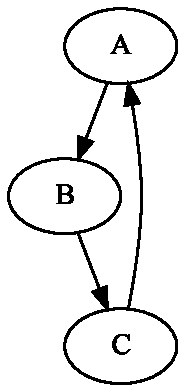
\includegraphics[width=4cm]{figures/example}
\caption{Some Example Figure generated from GRAPHVIZ DOT}\label{fig:intro:example}
\end{figure}

\marginnote{Note}
\lipsum[14]

\begin{figure}[htb]
\centering
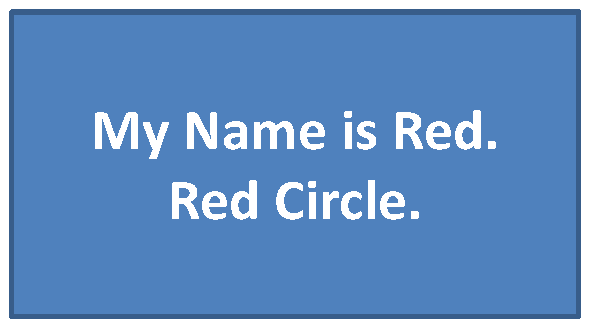
\includegraphics[width=\linewidth]{figures/example-pptx-figure}
\caption{Some Example Figure generated from a single PPTX Slide}\label{fig:intro:example2}
\end{figure}

\marginnote{Note}
\lipsum[15]

\appendix
\part{Appendix}

\chapter{Some Long Tables}
\lipsum[1]

\begin{table}[htb]
\scriptsize
\centering
\caption{Detailed Experiment Results}
\label{tab:appendix:engines:bpel}
\begin{tabular}{lrl}
	\toprule
\textbf{A} & \textbf{B} & \textbf{C} \\
\midrule
1 & 2 & 3 \\
1 & 2 & 3 \\
1 & 2 & 3 \\
1 & 2 & 3 \\
1 & 2 & 3 \\
1 & 2 & 3 \\
1 & 2 & 3 \\
1 & 2 & 3 \\
1 & 2 & 3 \\
1 & 2 & 3 \\
1 & 2 & 3 \\
1 & 2 & 3 \\
1 & 2 & 3 \\
1 & 2 & 3 \\
1 & 2 & 3 \\
1 & 2 & 3 \\
1 & 2 & 3 \\
\bottomrule
\end{tabular}
\end{table}

\bibliographystyle{IEEEtranSN}
\bibliography{references}

\end{document}
